\documentclass{standalone}
\usepackage{tikz}

\begin{document}

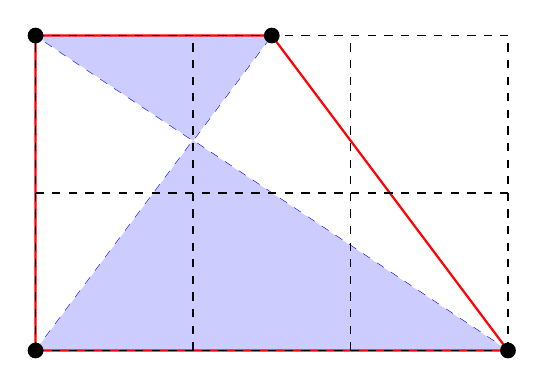
\begin{tikzpicture}[scale=2]
    % Define coordinates
    \coordinate (A) at (0,0);
    \coordinate (B) at (3,0);
    \coordinate (C) at (1.5,2);
    \coordinate (D) at (0,2);
    
    % Draw the main shape with dashed lines
    \draw[blue,dashed] (A) -- (B) -- (C) -- (D) -- cycle;
    \draw[blue,dashed] (A) -- (C);
    \draw[blue,dashed] (B) -- (D);
    
    % Fill the area with a pattern
    \fill[blue!20,even odd rule] 
        (A) -- (B) -- (C) -- (D) -- cycle 
        (A) -- (C) -- (B) -- (D) -- cycle;
    
    % Draw the red outline of the shape
    \draw[red, thick] (A) -- (B) -- (C) -- (D) -- cycle;
    
    % Add some grid lines for clarity
    \foreach \x in {0,...,3} {
        \draw[dashed] (\x,0) -- (\x,2);
    }
    \foreach \y in {0,...,2} {
        \draw[dashed] (0,\y) -- (3,\y);
    }
    
    % Add some small dots to indicate the corners
    \fill (A) circle (0.05);
    \fill (B) circle (0.05);
    \fill (C) circle (0.05);
    \fill (D) circle (0.05);
\end{tikzpicture}

\end{document}